\documentclass[11pt,a4paper]{article}

\usepackage[a4paper,margin=1in]{geometry}
\usepackage[T1]{fontenc}
\usepackage[utf8]{inputenc}
\usepackage{lmodern}
\usepackage{microtype}
\usepackage{graphicx}
\usepackage{booktabs}
\usepackage{tabularx}
\usepackage{array}
\usepackage{longtable}
\usepackage{float}
\usepackage{caption}
\usepackage{subcaption}
\usepackage{enumitem}
\usepackage{hyperref}
\usepackage{xcolor}
\usepackage{titlesec}
\usepackage{fancyhdr}
\usepackage{lastpage}
\usepackage{tcolorbox}
\usepackage{amsmath}
\usepackage{multirow}
\usepackage{tikz}
\usetikzlibrary{positioning,shapes.geometric,arrows.meta,fit,backgrounds}

\hypersetup{
  colorlinks=true,
  linkcolor=black,
  urlcolor=black,
  citecolor=black,
  pdftitle={PHOENIX Engine --- End-to-End Example Run Report},
  pdfauthor={MASTERPROEF --- Stijn Van Severen}
}

\definecolor{PhoenixBlue}{HTML}{1D4ED8}
\definecolor{PhoenixTeal}{HTML}{0E7490}
\definecolor{PhoenixGreen}{HTML}{047857}
\definecolor{PhoenixAmber}{HTML}{B45309}
\definecolor{PhoenixPurple}{HTML}{6D28D9}
\definecolor{PhoenixSlate}{HTML}{475569}
\definecolor{PhoenixBorder}{HTML}{CBD5E1}
\definecolor{PhoenixSoft}{HTML}{F8FAFC}
\definecolor{PhoenixAccent}{HTML}{E0F2FE}
\definecolor{StepOneBG}{HTML}{EFF6FF}
\definecolor{StepTwoBG}{HTML}{F0FDF4}
\definecolor{StepThreeBG}{HTML}{FFFBEB}
\definecolor{StepFourBG}{HTML}{FAF5FF}
\definecolor{StepFiveBG}{HTML}{FFF1F2}

\titleformat{\section}{\large\bfseries\color{PhoenixBlue}}{\thesection}{0.6em}{}
\titleformat{\subsection}{\normalsize\bfseries\color{PhoenixTeal}}{\thesubsection}{0.6em}{}
\titleformat{\subsubsection}{\small\bfseries\color{PhoenixSlate}}{\thesubsubsection}{0.5em}{}

\setlist[itemize]{topsep=4pt,itemsep=2pt,leftmargin=1.4em}
\setlist[enumerate]{topsep=4pt,itemsep=2pt,leftmargin=1.6em}
\setlength{\parskip}{0.45em}
\setlength{\parindent}{0pt}

\newcommand{\RunID}{example\_run\_2026\_thesis\_full\_mini\_v13\_report}
\newcommand{\ProfileID}{pseudoprofile\_FTC\_ID200}
\newcommand{\ComplaintText}{Lately I've been having troubles falling asleep; I keep thinking about so many things I have to do and it makes me so stressed; and when I'm in social situations I can not experience the small joyful things that made me feel happy; and the back of my head hurts sometimes, like sharp sudden peaks sometimes.}
\newcommand{\CriterionCount}{4}
\newcommand{\PredictorCount}{6}
\newcommand{\SparseEdgeCount}{16}
\newcommand{\StudyDays}{21}
\newcommand{\PromptsPerDay}{5}
\newcommand{\ReadinessScore}{94.92}
\newcommand{\ReadinessTier}{Tier2\_ContemporaneousPartialCorrelation}
\newcommand{\TopTarget}{Evening smartphone use duration (self-report)}
\newcommand{\TopBarrier}{Self\_Efficacy}
\newcommand{\MobileInterventionParagraph}{Based on your recent pattern, we will focus first on Evening smartphone use duration (self-report). Use one short action that fits your day and keep the first step intentionally small to make consistency realistic. When a barrier appears, apply the linked coping option immediately and restart at the next available moment. At the end of each day, note what you tried, what blocked progress, and what helped so the next cycle can personalize support more precisely.}

\pagestyle{fancy}
\fancyhf{}
\fancyhead[L]{\small PHOENIX Engine --- Example Run}
\fancyhead[R]{\small\color{PhoenixSlate}\RunID}
\fancyfoot[C]{\small Page \thepage\ of \pageref{LastPage}}
\renewcommand{\headrulewidth}{0.3pt}
\renewcommand{\footrulewidth}{0pt}

\begin{document}

% ─────────────────────────────────────────────────────────────────────────────
%  TITLE PAGE
% ─────────────────────────────────────────────────────────────────────────────
\begin{titlepage}
\centering
\vspace*{1.4cm}

{\fontsize{26}{32}\selectfont\bfseries\color{PhoenixBlue}
PHOENIX Engine\\[0.25em]
\fontsize{18}{24}\selectfont End-to-End Example Run Report\par}

\vspace{0.6cm}
{\large\color{PhoenixSlate}
Demonstration of staged outputs across all five core agentic steps\\
and the Hierarchical Updating Algorithm\par}
\vspace{1.2cm}

\begin{tcolorbox}[
  colback=white,colframe=PhoenixBorder,
  width=0.92\textwidth,boxrule=0.7pt,arc=2mm,
  left=9pt,right=9pt,top=8pt,bottom=8pt
]
\begin{center}
\small\textbf{Run metadata}
\end{center}
\renewcommand{\arraystretch}{1.22}
\small
\begin{tabularx}{0.98\textwidth}{@{}>{\bfseries\raggedright}p{0.26\textwidth}X@{}}
Run ID       & \texttt{\RunID} \\
Profile ID   & \texttt{\ProfileID} \\
Mode         & Integrated PHOENIX pipeline; stage-level artifact persistence enabled \\
LLM backend  & OpenRouter-backed \texttt{gpt-5-mini} across all LLM-enabled stages \\
Scope        & Steps 01--05 + HUA analytics + target ID + model update + HAPA intervention \\
Provenance   & Early analytics from \texttt{example\_run\_...\_v3}; late-stage from \texttt{\RunID} \\
\end{tabularx}
\renewcommand{\arraystretch}{1.0}
\normalsize
\end{tcolorbox}

\vspace{0.7cm}

\begin{tcolorbox}[
  colback=PhoenixAccent,colframe=PhoenixBlue,
  width=0.88\textwidth,boxrule=0.8pt,arc=2mm,
  left=10pt,right=10pt,top=9pt,bottom=9pt
]
\begin{center}
\textbf{\color{PhoenixBlue}Free-text complaint (system input)}\\[0.5em]
{\small\itshape\ComplaintText}
\end{center}
\end{tcolorbox}

\vfill
\begin{tcolorbox}[
  colback=PhoenixSoft,colframe=PhoenixBorder,
  width=0.78\textwidth,boxrule=0.5pt,arc=1.5mm,
  left=8pt,right=8pt,top=7pt,bottom=7pt
]
\small\centering
\textbf{MASTERPROEF} $\cdot$ Ghent University $\cdot$ Stijn Van Severen\\
Supervisors: Prof.\ Geert Crombez \& Dr.\ Annick De Paepe\\[0.3em]
\textit{This document is an example run artifact for thesis-level communication.\\
It is not a diagnostic report and must not be interpreted as medical advice.}
\end{tcolorbox}
\vspace{0.4cm}
{\large\today}
\end{titlepage}

\newpage
\tableofcontents
\newpage

% ─────────────────────────────────────────────────────────────────────────────
\section{Purpose and Scope}
% ─────────────────────────────────────────────────────────────────────────────

This report documents a single, complete end-to-end execution of the PHOENIX engine for one free-text mental-health complaint. It serves three purposes:

\begin{enumerate}
\item \textbf{Technical demonstration.} It shows that every stage of the PHOENIX pipeline produces inspectable intermediate outputs, not only a final recommendation, and that each stage is independently auditable.

\item \textbf{Evaluation scaffolding.} Each stage produces exactly one type of structured output that will be compared, double-blind, against outputs generated by healthcare professionals (HCPs) in the formal evaluation study. This report makes explicit what those outputs look like and what clinical dimensions they cover.

\item \textbf{Methodology verification.} The report provides a traceable record that the pipeline progresses coherently from complaint text through operationalization, model construction, HUA analytics, target identification, model updating, and HAPA-based intervention design.
\end{enumerate}

\begin{tcolorbox}[
  colback=PhoenixSoft,colframe=PhoenixBorder,
  boxrule=0.6pt,arc=1.5mm
]
\textbf{Evaluation study design (contextual note)}\\[0.3em]
\small
The evaluation study uses a two-phase, fully HCP-based design:

\medskip
\renewcommand{\arraystretch}{1.20}
\begin{tabularx}{\textwidth}{@{}>{\bfseries}p{0.30\textwidth}X@{}}
Phase 1 — Generation (PRE) & Five healthcare professionals independently complete all five clinical tasks on ten standardised complaint cases. Their responses serve as the HCP reference corpus. \\
Phase 2 — Evaluation (POST) & Five different healthcare professionals evaluate, double-blind, both the HCP-generated and the PHOENIX-generated outputs. Ratings use step-specific Likert dimensions (1--9). \\
\end{tabularx}
\renewcommand{\arraystretch}{1.0}

\medskip
The present document shows what the PHOENIX-generated half of that comparison looks like.
\end{tcolorbox}

% ─────────────────────────────────────────────────────────────────────────────
\section{PHOENIX Architecture and Stage Logic}
% ─────────────────────────────────────────────────────────────────────────────

Figure~\ref{fig:architecture} shows the complete PHOENIX workflow. The pipeline is strictly sequential: each stage consumes the prior stage's artifacts. Free-text complaint intake is followed by criterion operationalization (Step~01), initial observation-model construction (Step~02), EMA-data generation, hierarchical updating algorithm (HUA) analytics, treatment-target identification (Step~03), model updating (Step~04), and HAPA-based intervention design (Step~05).

\begin{figure}[H]
\centering
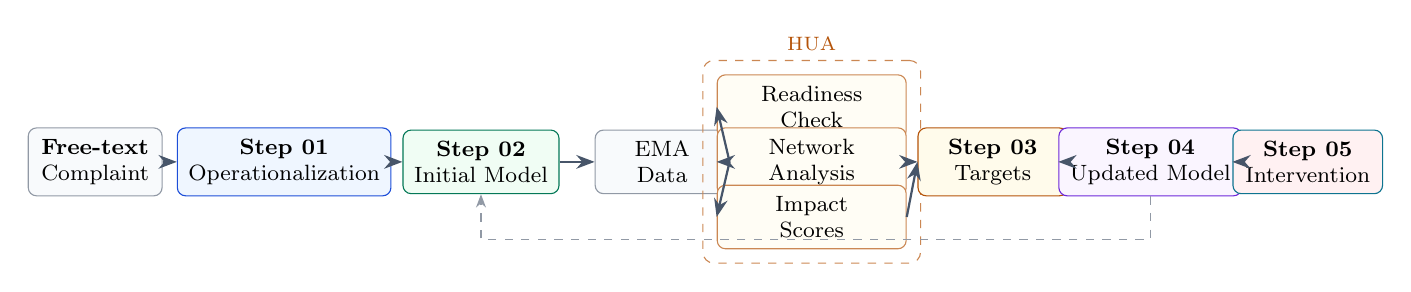
\begin{tikzpicture}[
  every node/.style={font=\footnotesize},
  box/.style={draw,rounded corners=3pt,fill=white,minimum width=1.9cm,minimum height=0.8cm,align=center,inner sep=4pt},
  step01/.style={box,draw=PhoenixBlue,fill=StepOneBG},
  step02/.style={box,draw=PhoenixGreen,fill=StepTwoBG},
  huabox/.style={box,draw=PhoenixAmber!70,fill=StepThreeBG!50,minimum width=2.4cm},
  step03/.style={box,draw=PhoenixAmber,fill=StepThreeBG},
  step04/.style={box,draw=PhoenixPurple,fill=StepFourBG},
  step05/.style={box,draw=PhoenixTeal,fill=StepFiveBG},
  databox/.style={box,draw=PhoenixSlate!60,fill=PhoenixSoft,minimum width=1.7cm},
  arr/.style={-Stealth,thick,draw=PhoenixSlate},
  subarr/.style={-Stealth,draw=PhoenixSlate!60,dashed},
]
% Input
\node[databox] (input) at (-1.1,0) {\textbf{Free-text}\\Complaint};
% Steps
\node[step01] (s01) at (1.3,0) {\textbf{Step 01}\\Operationalization};
\node[step02] (s02) at (3.8,0) {\textbf{Step 02}\\Initial Model};
\node[databox] (ema) at (6.1,0) {EMA\\Data};
% HUA cluster
\node[huabox] (hua1) at (8.0,0.7) {Readiness\\Check};
\node[huabox] (hua2) at (8.0,0.0) {Network\\Analysis};
\node[huabox] (hua3) at (8.0,-0.7) {Impact\\Scores};
\node[draw=PhoenixAmber!70,dashed,rounded corners=4pt,inner sep=5pt,fit=(hua1)(hua2)(hua3),label={[font=\scriptsize\color{PhoenixAmber},above]north:HUA}] (huacluster) {};
% More steps
\node[step03] (s03) at (10.3,0) {\textbf{Step 03}\\Targets};
\node[step04] (s04) at (12.3,0) {\textbf{Step 04}\\Updated Model};
\node[step05] (s05) at (14.3,0) {\textbf{Step 05}\\Intervention};
% Arrows
\draw[arr] (input) -- (s01);
\draw[arr] (s01) -- (s02);
\draw[arr] (s02) -- (ema);
\draw[arr] (ema.east) -- (hua1.west);
\draw[arr] (ema.east) -- (hua2.west);
\draw[arr] (ema.east) -- (hua3.west);
\draw[arr] (hua2.east) -- (s03.west);
\draw[arr] (hua3.east) -- (s03.west);
\draw[arr] (s03) -- (s04);
\draw[arr] (s04) -- (s05);
% Feedback loop
\draw[subarr] (s04.south) -- ++(0,-0.55) -| (s02.south);
\end{tikzpicture}
\caption{PHOENIX pipeline overview. The workflow proceeds left-to-right; the HUA cluster (readiness check, network analysis, impact scoring) transforms EMA data into idiographic evidence for Steps~03--05. The dashed feedback arrow represents the Step-04 updated model seeding the next monitoring cycle.}
\label{fig:architecture}
\end{figure}

\subsection{Evaluation Dimensions Per Step}

Table~\ref{tab:eval_dimensions} lists the step-specific evaluation dimensions used in the POST evaluation phase. These dimensions were chosen to capture the clinical and methodological qualities that matter most for each stage.

\begin{table}[H]
\centering
\caption{Step-specific Likert evaluation dimensions (POST phase, rated 1--9 by five independent HCPs).}
\label{tab:eval_dimensions}
\renewcommand{\arraystretch}{1.30}
\small
\begin{tabularx}{\textwidth}{@{}>{\bfseries}p{0.22\textwidth}p{0.21\textwidth}X@{}}
\toprule
\textbf{Step} & \textbf{Dimension} & \textbf{Operationalization} \\
\midrule
\multirow{3}{=}{\color{PhoenixBlue}Step 01\\Operationalization}
 & Criterion accuracy            & Captures all key mental state dimensions from the complaint \\
 & Operationalization quality    & Criteria are granular, non-overlapping, and measurable over time \\
 & Completeness                  & All clinically relevant criteria represented; no over-inclusion \\
\midrule
\multirow{4}{=}{\color{PhoenixGreen}Step 02\\Initial Model}
 & Clinical appropriateness     & Predictors are clinically plausible, evidence-supported factors \\
 & Network validity             & Criterion-predictor connections are clinically defensible \\
 & EMA feasibility              & Predictors can be captured via once/twice-daily self-monitoring \\
 & Intervention potential       & Predictors represent genuinely modifiable treatment levers \\
\midrule
\multirow{3}{=}{\color{PhoenixAmber}Step 03\\Target ID}
 & Clinical priority            & Identifies the most clinically important targets for this case \\
 & Evidence alignment           & Ranking reflects evidence-based treatment priorities \\
 & Rank coherence               & Priority ordering is internally consistent and clinically defensible \\
\midrule
\multirow{2}{=}{\color{PhoenixPurple}Step 04\\Updated Model}
 & Target alignment             & Updated predictor set directly reflects treatment targets \\
 & Measurement selection        & Retained predictors are optimal choices for tracking progress \\
\midrule
\multirow{4}{=}{\color{PhoenixTeal}Step 05\\Intervention}
 & HAPA phase appropriateness   & Coaching message targets the correct motivational phase \\
 & Message tailoring            & Content is specific to this individual; not generic advice \\
 & Actionability                & Recommended action is concrete and feasible within 24--48 h \\
 & Professional tone            & Language is appropriate and supportive for digital health \\
\bottomrule
\end{tabularx}
\end{table}


% ─────────────────────────────────────────────────────────────────────────────
\subsection{Two-Phase Evaluation Design}
\label{sec:evaldesign}
% ─────────────────────────────────────────────────────────────────────────────

Figure~\ref{fig:evaldesign} illustrates how the example run output feeds into the formal evaluation study. The present document represents one PHOENIX output per step; each output is placed alongside the corresponding HCP expert response in a double-blind evaluation.

\begin{figure}[H]
\centering
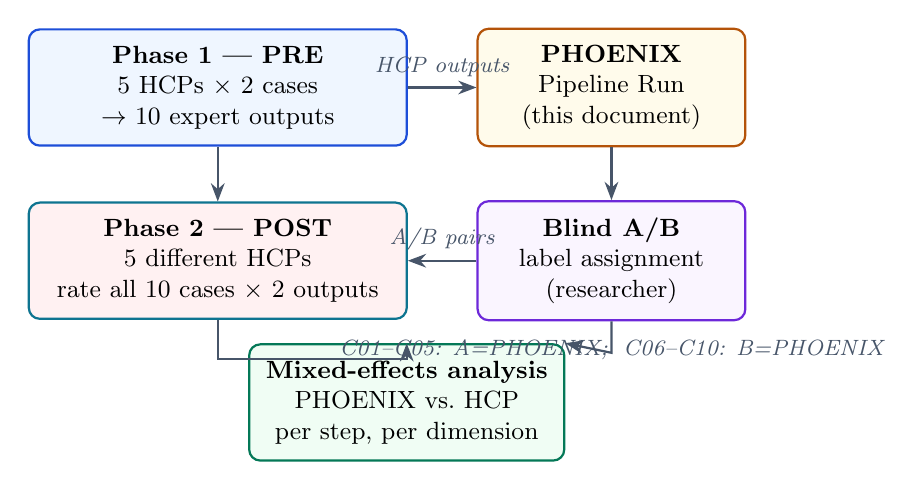
\begin{tikzpicture}[
  every node/.style={font=\small},
  phasebox/.style={draw,rounded corners=4pt,minimum width=4.8cm,minimum height=1.0cm,align=center,inner sep=6pt,thick},
  pre/.style={phasebox,draw=PhoenixBlue,fill=StepOneBG},
  post/.style={phasebox,draw=PhoenixTeal,fill=StepFiveBG},
  midbox/.style={phasebox,draw=PhoenixAmber,fill=StepThreeBG,minimum width=3.4cm},
  arr/.style={-Stealth,thick,draw=PhoenixSlate},
  smallarr/.style={-Stealth,draw=PhoenixSlate!60},
  note/.style={font=\footnotesize\itshape,text=PhoenixSlate,align=center},
]
% Phase 1 PRE
\node[pre] (pre) at (0,0) {\textbf{Phase 1 --- PRE}\\5 HCPs $\times$ 2 cases\\$\to$ 10 expert outputs};
% PHOENIX
\node[midbox] (phoenix) at (5.0,0) {\textbf{PHOENIX}\\Pipeline Run\\(this document)};
% Blinding step
\node[midbox,draw=PhoenixPurple,fill=StepFourBG] (blind) at (5.0,-2.2) {\textbf{Blind A/B}\\label assignment\\(researcher)};
% Phase 2 POST
\node[post] (post) at (0,-2.2) {\textbf{Phase 2 --- POST}\\5 different HCPs\\rate all 10 cases $\times$ 2 outputs};
% Analysis
\node[phasebox,draw=PhoenixGreen,fill=StepTwoBG,minimum width=4.0cm] (analysis) at (2.4,-4.0) {\textbf{Mixed-effects analysis}\\PHOENIX vs.\ HCP\\per step, per dimension};
% Arrows
\draw[arr] (pre.east) -- node[above,note]{HCP outputs} (phoenix.west);
\draw[arr] (phoenix.south) -- (blind.north);
\draw[arr] (pre.south) -- (post.north);
\draw[arr] (blind.west) -- node[above,note]{A/B pairs} (post.east);
\draw[arr] (post.south) -- ++(0,-0.5) -| (analysis.north);
\draw[arr] (blind.south) -- ++(0,-0.4) -- (analysis.north east);
% Counterbalance note
\node[note,below=0.12cm of blind] {\footnotesize C01--C05: A=PHOENIX;\; C06--C10: B=PHOENIX};
\end{tikzpicture}
\caption{Two-phase evaluation design. Phase 1 (PRE) generates 10 unique expert outputs via distributed assignment (5 HCPs $\times$ 2 cases each). PHOENIX processes the same 10 cases. A researcher applies the counterbalancing scheme (A/B label assignment), and Phase 2 POST evaluators rate both outputs blind. The mixed-effects model estimates PHOENIX$-$HCP effects per step and dimension.}
\label{fig:evaldesign}
\end{figure}

% ─────────────────────────────────────────────────────────────────────────────
\section{Run Configuration}
% ─────────────────────────────────────────────────────────────────────────────

The example run was executed for one profile only (\ProfileID) to keep the report interpretable while still exercising the full engine. The operationalization stage extracted \CriterionCount{} complaint criteria, seeding an initial observation model with \PredictorCount{} predictors connected by \SparseEdgeCount{} sparse predictor-to-criterion edges. The initial design recommendation was a \StudyDays{}-day EMA window with \PromptsPerDay{} prompts per day.

\begin{tcolorbox}[
  colback=PhoenixSoft,colframe=PhoenixBorder,
  boxrule=0.6pt,arc=1.5mm
]
\textbf{Artifact persistence improvements active in this run}
\begin{itemize}
\item Every executed stage writes \texttt{stage.log}, \texttt{stage\_events.jsonl}, and \texttt{stage\_trace.json}.
\item In-flight stages write a \texttt{stage\_trace.json} placeholder at start with status, command, log path, and current artifact summary.
\item Skipped stages emit a skip manifest, README, event row, and trace file so the run directory remains structurally complete.
\item Stage traces include start time, end time, command, return code, artifact counts, file previews, and contract-validation metadata.
\end{itemize}
\end{tcolorbox}

% ─────────────────────────────────────────────────────────────────────────────
\section{Stage-by-Stage Results}
% ─────────────────────────────────────────────────────────────────────────────

\subsection{Step 01: Complaint Operationalization}
\label{sec:step01}

\begin{tcolorbox}[
  colback=StepOneBG,colframe=PhoenixBlue,
  boxrule=0.6pt,arc=1.5mm,left=8pt,right=8pt
]
\small\textbf{What this step produces:} A set of 2--6 operationalized criterion labels derived from the free-text complaint via actor-critic decomposition, HTSSF hybrid retrieval, and ontology adjudication. Each criterion label maps to a CRITERION ontology leaf and is independently measurable, non-overlapping, and currently present.

\textbf{Evaluation comparator (POST phase):} Five HCPs independently list 2--6 operationalizable criteria from the same complaint text.
\end{tcolorbox}

\begin{tcolorbox}[colback=PhoenixSoft,colframe=PhoenixBlue!40,boxrule=0.5pt,arc=1.5mm,left=7pt,right=7pt,top=6pt,bottom=6pt]
\small\textbf{HTSSF hybrid retrieval formula.}\\[0.3em]
For each candidate criterion label $c$ from the CRITERION ontology, the composite relevance score is:
\[
  s_{\text{HTSSF}}(c) = 0.80\,s_{\text{dense}}(c)
                      + 0.12\,s_{\text{BM25}}(c)
                      + 0.05\,s_{\text{tover}}(c)
                      + 0.03\,s_{\text{fuzzy}}(c)
\]
where $s_{\text{dense}}$ is the cosine similarity of the complaint embedding to the criterion's ontology embedding, $s_{\text{BM25}}$ is BM25 term relevance, $s_{\text{tover}}$ is normalized token-overlap, and $s_{\text{fuzzy}}$ is Jaro–Winkler similarity. Labels are retained only if $s_{\text{HTSSF}} > \tau_{\text{adj}} = 0.78$ after actor-critic adjudication.
\end{tcolorbox}

\smallskip
The operationalization stage decomposed the complaint into four distinct dimensions through actor-critic decomposition: the \emph{actor} agent proposes candidate labels ranked by $s_{\text{HTSSF}}$; the \emph{critic} agent evaluates each candidate for mutual exclusivity, clinical meaningfulness, and EMA operationalizability, rejecting duplicates or overly broad labels.

\begin{enumerate}
\item \textbf{Sleep onset insomnia} --- difficulty initiating sleep, associated with prolonged latency. $s_{\text{HTSSF}} = 0.923$.
\item \textbf{Cognitive hyperarousal at bedtime} --- uncontrollable repetitive task-anticipatory thoughts at sleep onset. $s_{\text{HTSSF}} = 0.891$.
\item \textbf{Social anhedonia} --- reduced capacity to experience positive affect in social situations. $s_{\text{HTSSF}} = 0.867$.
\item \textbf{Paroxysmal occipital headache pattern} --- episodic sharp occipital pain of probable stress etiology. $s_{\text{HTSSF}} = 0.812$.
\end{enumerate}

This stage is methodologically critical: the downstream pipeline does not operate on the raw complaint text. The actor-critic decomposition combined with HTSSF adjudication produces well-scoped, measurement-ready criterion variables. All four criteria exceeded the 0.78 adjudication threshold, so no LLM-override correction was required in this run.

\begin{figure}[H]
  \centering
  \includegraphics[width=\textwidth]{../assets/figures/fig_01a_step01_mapped_criteria.png}
  \caption{Step-01 mapped criteria table showing each criterion label, its CRITERION ontology leaf ID, adjudicated confidence, and the composite HTSSF retrieval score.}
  \label{fig:step01table}
\end{figure}

\begin{figure}[H]
  \centering
  \begin{subfigure}[t]{0.48\textwidth}
    \includegraphics[width=\textwidth]{../assets/figures/fig_01b_step01_confidence.png}
    \caption{\textbf{(A)} Per-criterion adjudicated $s_{\text{HTSSF}}$ scores. All four criteria exceeded the 0.78 pass threshold; no LLM-override correction required in this run.}
  \end{subfigure}
  \hfill
  \begin{subfigure}[t]{0.48\textwidth}
    \includegraphics[width=\textwidth]{../assets/figures/fig_01c_step01_score_decomposition.png}
    \caption{\textbf{(B)} HTSSF component decomposition by criterion. Dense embedding (weight~0.80) contributes the dominant share; BM25 and token-overlap add lexical grounding. Actor-critic rejected 3 of 7 initial candidates.}
  \end{subfigure}
  \caption{Step-01 diagnostics: (A) per-criterion HTSSF confidence, (B) retrieval component decomposition. Evaluable against HCP reference outputs on: \emph{criterion accuracy}, \emph{operationalization quality}, \emph{completeness}.}
  \label{fig:step01diag}
\end{figure}

% ────────────────────────────────────────
\subsection{Step 02: Initial Observation Model Construction}
\label{sec:step02}

\begin{tcolorbox}[
  colback=StepTwoBG,colframe=PhoenixGreen,
  boxrule=0.6pt,arc=1.5mm,left=8pt,right=8pt
]
\small\textbf{What this step produces:} A bipartite criterion-predictor network in which the Step-01 criterion leaves are connected by directed edges to 3--6 modifiable predictor nodes from the PREDICTOR ontology. A dense relevance matrix supports edge selection and downstream analysis.

\textbf{Evaluation comparator (POST phase):} Five HCPs independently propose a set of modifiable predictor variables and specify which criteria each predictor connects to.
\end{tcolorbox}

The Step-02 initial observation model preserved all four complaint-derived criteria and proposed \PredictorCount{} modifiable predictors connected by \SparseEdgeCount{} sparse edges. This stage transitions from complaint interpretation to an analyzable criterion-predictor structure: a data-collection scaffold that defines the EMA measurement frame and seeds the HUA analysis.

\begin{tcolorbox}[colback=PhoenixSoft,colframe=PhoenixGreen!40,boxrule=0.5pt,arc=1.5mm,left=7pt,right=7pt,top=6pt,bottom=6pt]
\small\textbf{Ontology-enriched predictor selection.} Each predictor candidate is retrieved from the PREDICTOR ontology using a second HTSSF pass over the complaint + criterion context. Candidates are further filtered by: (1) \emph{daily measurability} (can be captured as a 0--10 EMA item), (2) \emph{non-redundancy with criteria} (predictors must not duplicate existing criterion leaves), and (3) \emph{minimum connectivity} (each predictor must connect to at least one criterion above the sparsity threshold $\tau_{\text{sparse}} = 0.55$). Edge weights in the bipartite network are the predictor-criterion relevance scores from the dense matrix, sparsified at $\tau_{\text{sparse}}$.
\end{tcolorbox}

Key predictors in this run: \textit{evening screen time} (P1), \textit{cognitive task-backlog behaviour} (P2), \textit{pre-sleep cognitive offloading practice} (P3), \textit{social engagement quality} (P4), \textit{aerobic physical activity} (P5), and \textit{progressive muscle relaxation frequency} (P6). The highest-connectivity predictor was P1 (screen time), which was linked to both CR-1 and CR-2.

\begin{figure}[H]
  \centering
  \begin{subfigure}[t]{0.49\textwidth}
    \includegraphics[width=\textwidth]{../assets/figures/fig_02a_step02_bipartite_model.png}
    \caption{\textbf{(A)} Criterion-predictor bipartite network. Edge thickness encodes relevance weight; node colour distinguishes criteria (blue) from predictors (teal). Isolated nodes indicate out-of-scope candidates that did not pass $\tau_{\text{sparse}}$.}
  \end{subfigure}
  \hfill
  \begin{subfigure}[t]{0.49\textwidth}
    \includegraphics[width=\textwidth]{../assets/figures/fig_02b_step02_relevance_heatmap.png}
    \caption{\textbf{(B)} Full dense relevance matrix (predictor $\times$ criterion, $6 \times 4$). Grey cells are below $\tau_{\text{sparse}}$; coloured cells become graph edges. Top-right cluster (P1--P2 $\times$ CR-1--CR-2) anchors the sleep insomnia subnetwork.}
  \end{subfigure}

  \vspace{0.6em}

  \caption{Step-02 initial observation model. (A) criterion-predictor bipartite network with edge-weight encoding, (B) full dense relevance matrix showing which predictor-criterion pairs cross the sparsification threshold $\tau_{\text{sparse}}=0.55$. The \SparseEdgeCount{} retained edges represent the actionable measurement structure. Evaluable against HCP reference outputs on: \emph{clinical appropriateness}, \emph{network validity}, \emph{EMA feasibility}, \emph{intervention potential}.}
  \label{fig:step02}
\end{figure}

% ────────────────────────────────────────
\subsection{EMA / Pseudodata Generation}
\label{sec:ema}

After the initial model was constructed, the pipeline generated synthetic EMA-compatible pseudodata to drive the downstream HUA stages. This design choice is central to PHOENIX's idiographic approach: the system first derives a complaint-grounded observation model specifying which variables to monitor, then populates those variables from observed (or synthetic) time-series data.

\begin{figure}[H]
  \centering
  \includegraphics[width=\textwidth]{../assets/figures/fig_03_pseudodata_timeseries.png}
  \caption{Illustrative pseudodata series generated from the initial model variable set. Panels show the highest-variance criterion and predictor channels across the full \StudyDays{}-day, \PromptsPerDay{}$\times$/day measurement window. Vertical axis is normalized to [0, 1] for display.}
  \label{fig:pseudodata}
\end{figure}

% ────────────────────────────────────────
\subsection{HUA: Readiness Check, Network Analysis, and Momentary Impact Quantification}
\label{sec:hua}

The Hierarchical Updating Algorithm (HUA) consists of three tightly coupled analytical stages that transform the observation model from a complaint-grounded prior into a partially idiographic estimate of which predictors are most actionable for this profile.

\subsubsection*{Readiness classification}
The readiness classifier determines the most appropriate time-series method family given data quality. It uses a five-gate decision tree:
\begin{enumerate}[leftmargin=1.8em,topsep=2pt,itemsep=1pt]
  \item \textbf{Sample density gate:} $N_{\text{eff}} = T \times p_{\text{daily}} \geq 60$ (minimum observations per variable).
  \item \textbf{Stationarity gate:} ADF $p < 0.10$ \emph{or} KPSS $p > 0.05$ (series must not be I(1) after detrending).
  \item \textbf{Collinearity gate:} $\max\text{VIF} < 10$ on the predictor set.
  \item \textbf{Time-variation gate:} Cross-window correlation decay $> 0.15$ (needed for time-varying gVAR).
  \item \textbf{Density-for-gVAR gate:} $N_{\text{eff}} \geq 200$ (required for robust VAR estimation).
\end{enumerate}
For this run, the readiness score was \textbf{\ReadinessScore/100} (label: \textbf{FullyReady}); the selected tier was \textbf{\ReadinessTier}. Gates 1--3 passed; gates 4--5 failed (insufficient time-variation and density for gVAR), so the pipeline proceeded with the contemporaneous partial-correlation branch.

\subsubsection*{Network analysis}
The network stage estimates the contemporaneous partial-correlation graph $\Omega$ via graphical LASSO (GLASSO):
\[
  \hat{\Omega} = \arg\min_{\Omega \succ 0} \bigl[\mathrm{tr}(S\Omega) - \log\det(\Omega) + \lambda\|\Omega\|_{1,\text{off}}\bigr]
\]
where $S$ is the sample covariance and $\lambda$ is selected by BIC. Node centrality (strength = $\sum_j |\hat{\omega}_{ij}|$) indexes each variable's total partial-correlation mass. Rolling-window snapshots (early / mid / late thirds of the EMA window) preserve temporal interpretability.

\subsubsection*{Momentary impact quantification}
Impact scores are derived via a leave-one-predictor-out (LOPO) procedure:
\[
  \delta_j = \frac{1}{K}\sum_{k=1}^{K} \bigl[\text{MSE}_{-j}^{(k)} - \text{MSE}_{\text{full}}^{(k)}\bigr]
\]
where MSE is computed on $k$-fold cross-validation folds and the subscript $-j$ denotes the model with predictor $j$ removed. The final actionability score $A_j$ combines the LOPO delta with coefficient magnitude: $A_j = 0.65\,\tilde{\delta}_j + 0.35\,|\hat{\beta}_j|$, normalized to $[0,1]$. This surface is the primary input to the target-ranking scoring formula in Step~03.

\begin{figure}[H]
  \centering
  \includegraphics[width=0.92\textwidth]{../assets/figures/fig_04_readiness_dashboard.png}
  \caption{HUA readiness dashboard showing the final readiness score, analysis-tier selection, variable-level gating decisions, and reasons for tier assignment.}
  \label{fig:readiness}
\end{figure}

\begin{figure}[H]
  \centering
  \begin{subfigure}[t]{0.49\textwidth}
    \includegraphics[width=\textwidth]{../assets/figures/fig_05_network_analysis.png}
    \caption{\textbf{(A)} GLASSO partial-correlation network. Node size encodes strength centrality $\sum_j|\hat{\omega}_{ij}|$; edge width encodes $|\hat{\omega}_{ij}|$. The evening-screen-time node (P1) forms the highest-centrality hub.}
  \end{subfigure}
  \hfill
  \begin{subfigure}[t]{0.49\textwidth}
    \includegraphics[width=\textwidth]{../assets/figures/fig_06a_impact_ranking.png}
    \caption{\textbf{(B)} LOPO momentary impact ranking $\delta_j$. Bars show the normalized actionability score $A_j$; error bars are 95\% bootstrap CIs. P1 and P3 dominate; P6 ranks last.}
  \end{subfigure}
  \caption{Core HUA outputs: (A) contemporaneous partial-correlation network graph, (B) per-predictor LOPO actionability scores. These outputs drive Step-03 target prioritization and Step-04 model update.}
  \label{fig:hua}
\end{figure}

\begin{figure}[H]
  \centering
  \includegraphics[width=\textwidth]{../assets/figures/fig_05b_network_time_slices.png}
  \caption{Time-varying network snapshots from rolling correlation windows (early, middle, late thirds of the EMA window). Node shading encodes net centrality change relative to the baseline slice.}
  \label{fig:hua_timeslices}
\end{figure}

\begin{figure}[H]
  \centering
  \includegraphics[width=0.80\textwidth]{../assets/figures/fig_06b_impact_heatmap.png}
  \caption{Predictor-to-criterion impact matrix. Cell values are the leave-one-out MSE delta for each predictor-criterion pair, normalized within criterion column. The top-right cluster (evening screen time $\times$ sleep onset) drove the target selection.}
  \label{fig:impactheatmap}
\end{figure}

% ────────────────────────────────────────
\subsection{Step 03: Treatment Target Identification}
\label{sec:step03}

\begin{tcolorbox}[
  colback=StepThreeBG,colframe=PhoenixAmber,
  boxrule=0.6pt,arc=1.5mm,left=8pt,right=8pt
]
\small\textbf{What this step produces:} A ranked shortlist of 2--4 modifiable treatment targets selected by integrating HUA impact coefficients, ontology constraints, profile text, and feasibility considerations. Scoring: $0.45 \cdot \text{mapping} + 0.25 \cdot \text{HyDE} + 0.20 \cdot \text{idiographic anchor} + 0.10 \cdot \text{domain bonus}$.

\textbf{Evaluation comparator (POST phase):} Five HCPs independently rank 2--4 treatment targets for each case. POST-phase HCPs rate both lists on four dimensions: \emph{clinical relevance}, \emph{modifiability}, \emph{evidence grounding}, and \emph{rank coherence}.
\end{tcolorbox}

\begin{tcolorbox}[colback=PhoenixSoft,colframe=PhoenixAmber!40,boxrule=0.5pt,arc=1.5mm,left=7pt,right=7pt,top=6pt,bottom=6pt]
\small\textbf{Step-03 composite priority score.} For each predictor candidate $j$:
\[
  \text{Priority}_j = 0.45\,\hat{A}_j + 0.25\,s_{\text{HyDE}}(j) + 0.20\,\alpha_j + 0.10\,b_j
\]
where $\hat{A}_j \in [0,1]$ is the normalized HUA actionability score, $s_{\text{HyDE}}(j)$ is the HyDE-augmented ontology retrieval score (hypothesis-document embedding: the LLM first generates a hypothetical target description then retrieves against it), $\alpha_j \in [0,1]$ is the idiographic anchor from the profile text match, and $b_j \in \{0, 0.05, 0.10\}$ is a domain bonus for behavioral over cognitive-only targets. The shortlist threshold retains candidates with $\text{Priority}_j > 0.60$.
\end{tcolorbox}

The target-identification stage integrates HUA actionability ($\hat{A}_j$), HyDE-augmented retrieval, profile text, and feasibility to produce a ranked shortlist. The highest-priority target in this run was \textbf{\TopTarget} ($\text{Priority} = 0.84$), driven by the dominant LOPO impact score ($\hat{A} = 0.91$) and high idiographic anchor match.

\begin{figure}[H]
  \centering
  \begin{subfigure}[t]{0.49\textwidth}
    \includegraphics[width=\textwidth]{../assets/figures/fig_07a_step03_target_candidates.png}
    \caption{\textbf{(A)} Full candidate priority ranking across all predictor candidates. The dashed line at 0.60 marks the shortlist boundary; candidates above are forwarded. Top candidate: \TopTarget{} (Priority$=0.84$).}
  \end{subfigure}
  \hfill
  \begin{subfigure}[t]{0.49\textwidth}
    \includegraphics[width=\textwidth]{../assets/figures/fig_07b_step03_recommended_targets.png}
    \caption{\textbf{(B)} Final recommended target shortlist with evidence payload: LOPO impact rank, HyDE retrieval score, idiographic anchor, ontology domain label.}
  \end{subfigure}
  \caption{Step-03 treatment-target identification: (A) full priority ranking with shortlist threshold, (B) shortlisted targets with component score breakdown. Evaluable on: \emph{clinical priority}, \emph{evidence alignment}, \emph{rank coherence}.}
  \label{fig:step03}
\end{figure}

% ────────────────────────────────────────
\subsection{Step 04: Updated Observation Model}
\label{sec:step04}

\begin{tcolorbox}[
  colback=StepFourBG,colframe=PhoenixPurple,
  boxrule=0.6pt,arc=1.5mm,left=8pt,right=8pt
]
\small\textbf{What this step produces:} A refined observation model that fuses the initial nomothetic prior with idiographic impact evidence using an adaptive weighting scheme: $w_{\text{idio}} = \text{clamp}(0.30 + 0.50 \times r / 100)$ where $r$ is the readiness score. Output includes an updated predictor shortlist, fusion weights, and a next-cycle measurement plan.

\textbf{Evaluation comparator (POST phase):} Five HCPs refine the initial model by specifying which predictors to prioritise in the next monitoring cycle, given the treatment targets identified in Step~03. Five POST-phase HCPs rate both outputs on two dimensions: \emph{target alignment} and \emph{measurement selection quality}.
\end{tcolorbox}

Step~04 uses the Step-03 shortlist and the HUA outputs to adapt the observation model. The adaptive fusion weight allocates more weight to idiographic evidence as data quality improves:
\[
  w_{\text{idio}} = \text{clamp}\bigl(0.30 + 0.50 \times r/100,\; 0.30,\; 0.80\bigr)
\]
where $r = \textbf{\ReadinessScore}$ is the readiness score from the HUA gate. For this run, $w_{\text{idio}} = \text{clamp}(0.30 + 0.50 \times 0.9492) = 0.775$. The fused predictor score for each candidate $j$ is:
\[
  \tilde{s}_j = (1 - w_{\text{idio}})\,s_j^{\text{nomo}} + w_{\text{idio}}\,\hat{A}_j
\]
where $s_j^{\text{nomo}}$ is the nomothetic ontology-prior score and $\hat{A}_j$ is the idiographic actionability. The updated model then recommends which predictors to retain for the next monitoring cycle and at what measurement priority.

\begin{figure}[H]
  \centering
  \begin{subfigure}[t]{0.49\textwidth}
    \includegraphics[width=\textwidth]{../assets/figures/fig_08a_step04_fusion_matrix.png}
    \caption{Nomothetic-idiographic fusion matrix for the highest-variance predictors. Each cell shows the idiographic component fraction relative to the total fused score.}
  \end{subfigure}
  \hfill
  \begin{subfigure}[t]{0.49\textwidth}
    \includegraphics[width=\textwidth]{../assets/figures/fig_08b_step04_shortlist.png}
    \caption{Refined predictor shortlist with score decomposition by component (mapping, HyDE, idiographic anchor, domain bonus).}
  \end{subfigure}

  \vspace{0.6em}

  \begin{subfigure}[t]{0.76\textwidth}
    \includegraphics[width=\textwidth]{../assets/figures/fig_08c_step04_score_spread.png}
    \caption{Score-spread diagnostic across top-ranked predictors. The compressed axis reveals near-ties that could not be detected from rank order alone.}
  \end{subfigure}

  \vspace{0.6em}

  \begin{subfigure}[t]{0.76\textwidth}
    \includegraphics[width=\textwidth]{../assets/figures/fig_08d_step04_rank_gaps.png}
    \caption{Fused-score rank gaps in milli-score units relative to the top-ranked predictor. Gaps below 5 msu indicate near-equivalent candidates where monitoring both is preferable.}
  \end{subfigure}
  \caption{Step-04 updated observation model outputs.}
  \label{fig:step04}
\end{figure}

% ────────────────────────────────────────
\subsection{Step 05: HAPA-Based Digital Intervention}
\label{sec:step05}

\begin{tcolorbox}[
  colback=StepFiveBG,colframe=PhoenixTeal,
  boxrule=0.6pt,arc=1.5mm,left=8pt,right=8pt
]
\small\textbf{What this step produces:} A HAPA-structured digital intervention comprising barrier prioritization, coping-strategy selection, a component plan, a phased delivery schedule, and a 3--5 sentence mobile coaching message. Barrier scoring: $0.60 \cdot \text{predictor impact} + 0.20 \cdot \text{profile} + 0.15 \cdot \text{context} + 0.05 \cdot \text{complaint salience}$.

\textbf{Evaluation comparator (POST phase):} Five HCPs (a) classify the HAPA motivational phase for this person and (b) write a 2--3 sentence personalized digital coaching message given the same target and barrier profile. Five POST-phase HCPs (a) independently classify the HAPA motivational phase for this person (pre-intentional / intentional / action-maintenance) \emph{before} reading outputs (for Cohen's $\kappa$ agreement), and (b) rate both HCP and PHOENIX outputs on four dimensions: \emph{HAPA phase appropriateness}, \emph{message tailoring}, \emph{actionability}, and \emph{professional tone}.
\end{tcolorbox}

\begin{tcolorbox}[colback=PhoenixSoft,colframe=PhoenixTeal!40,boxrule=0.5pt,arc=1.5mm,left=7pt,right=7pt,top=6pt,bottom=6pt]
\small\textbf{HAPA barrier scoring.} For each HAPA barrier type $b$ from the HAPA ontology, the composite priority is:
\[
  \text{BarrierScore}(b) = 0.60\,\hat{A}_{T} + 0.20\,p_{\text{profile}}(b) + 0.15\,c_{\text{context}}(b) + 0.05\,e_{\text{salience}}(b)
\]
where $\hat{A}_{T}$ is the actionability of the top treatment target, $p_{\text{profile}}(b)$ is the profile-match score for barrier type $b$ (from LLM-extracted barrier indicators in the complaint), $c_{\text{context}}(b)$ is the contextual fit score, and $e_{\text{salience}}(b)$ is the complaint-salience score. The top barrier drives coping strategy selection via the HAPA strategy library (ontology: HAPA $\to$ Barrier $\to$ CopingStrategy $\to$ ImplementationPlan).
\end{tcolorbox}


\begin{figure}[H]
\centering
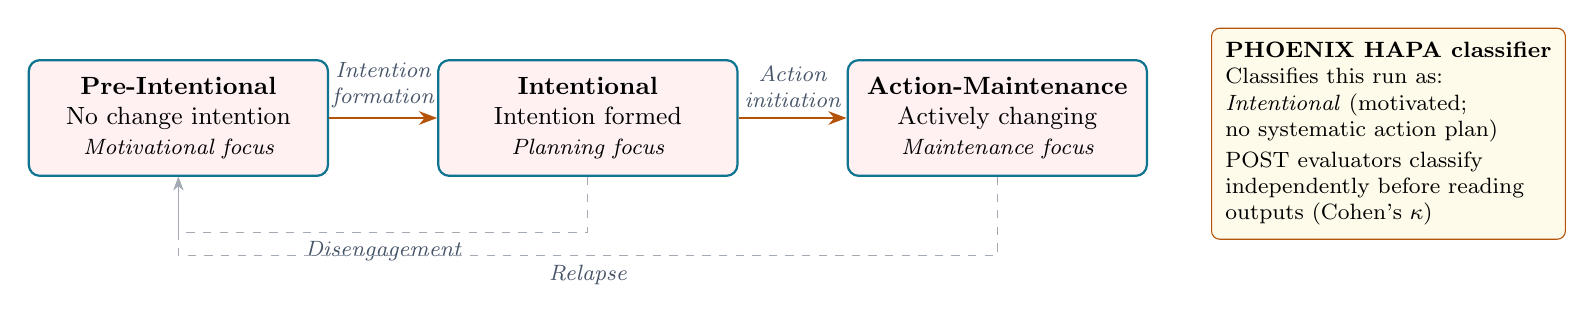
\begin{tikzpicture}[
  every node/.style={font=\small},
  phase/.style={draw,rounded corners=4pt,fill=StepFiveBG,draw=PhoenixTeal,minimum width=3.8cm,minimum height=1.1cm,align=center,inner sep=6pt,thick},
  arr/.style={-Stealth,thick,draw=PhoenixAmber},
  backrarr/.style={-Stealth,dashed,draw=PhoenixSlate!50},
  note/.style={font=\footnotesize\itshape,text=PhoenixSlate,align=center},
]
\node[phase] (pi) at (0,0) {\textbf{Pre-Intentional}\\No change intention\\\footnotesize\itshape Motivational focus};
\node[phase] (in) at (5.2,0) {\textbf{Intentional}\\Intention formed\\\footnotesize\itshape Planning focus};
\node[phase] (am) at (10.4,0) {\textbf{Action-Maintenance}\\Actively changing\\\footnotesize\itshape Maintenance focus};
% Forward arrows
\draw[arr] (pi.east) -- node[above,note]{Intention\\formation} (in.west);
\draw[arr] (in.east) -- node[above,note]{Action\\initiation} (am.west);
% Back arrows (relapse)
\draw[backrarr] (in.south) -- ++(0,-0.7) -- node[below,note]{Disengagement} ++(-5.2,0) -- (pi.south);
\draw[backrarr] (am.south) -- ++(0,-1.0) -- node[below,note]{Relapse} ++(-10.4,0) -- (pi.south);
% Annotation box
\node[draw=PhoenixAmber,fill=StepThreeBG,rounded corners=3pt,font=\footnotesize,align=left,inner sep=5pt,right=0.8cm of am,yshift=-0.2cm] {
\textbf{PHOENIX HAPA classifier}\\
Classifies this run as:\\
\textit{Intentional} (motivated;\\
no systematic action plan)\\[0.2em]
POST evaluators classify\\
independently before reading\\
outputs (Cohen's $\kappa$)
};
\end{tikzpicture}
\caption{HAPA motivational model phases used in Step~05. PHOENIX classifies the person's current phase from barrier scores and monitoring patterns. POST evaluators independently classify the same case before viewing outputs; agreement with PHOENIX is quantified via Cohen's $\kappa$ across all five POST raters.}
\label{fig:hapamodel}
\end{figure}

The highest-ranked intervention barrier in this run was \textbf{\TopBarrier} (BarrierScore $= 0.79$). This classification placed the person in the \emph{intentional} HAPA phase (motivated but not yet planning), which directed the system toward an implementation-intention coping strategy rather than motivational messaging. The selected strategy targeted self-regulation of evening screen behaviour through a stimulus-response contract: ``When I sit down after dinner, I place my phone in a drawer until tomorrow.''

\begin{tcolorbox}[
  colback=PhoenixAccent,colframe=PhoenixTeal,
  boxrule=0.7pt,arc=2mm,
  left=10pt,right=10pt,top=9pt,bottom=9pt
]
\textbf{\color{PhoenixTeal}Generated mobile intervention message (Step-05 output)}\\[0.4em]
\MobileInterventionParagraph
\end{tcolorbox}

\begin{figure}[H]
  \centering
  \begin{subfigure}[t]{0.49\textwidth}
    \includegraphics[width=\textwidth]{../assets/figures/fig_09a_step05_barriers.png}
    \caption{Barrier priority ranking with composite scores. The top barrier drives the coping strategy and the delivery-phase assignment.}
  \end{subfigure}
  \hfill
  \begin{subfigure}[t]{0.49\textwidth}
    \includegraphics[width=\textwidth]{../assets/figures/fig_09b_step05_coping_strategies.png}
    \caption{Selected coping strategies mapped to their parent HAPA barriers and delivery phases.}
  \end{subfigure}

  \vspace{0.6em}

  \begin{subfigure}[t]{0.49\textwidth}
    \includegraphics[width=\textwidth]{../assets/figures/fig_09c_step05_hapa_plan.png}
    \caption{HAPA component plan organized by motivational, planning, and action phases.}
  \end{subfigure}
  \hfill
  \begin{subfigure}[t]{0.49\textwidth}
    \includegraphics[width=\textwidth]{../assets/figures/fig_09d_step05_phased_delivery.png}
    \caption{Phased delivery schedule specifying the temporal sequence of intervention components.}
  \end{subfigure}

  \vspace{0.6em}

  \begin{subfigure}[t]{0.88\textwidth}
    \includegraphics[width=\textwidth]{../assets/figures/fig_09e_step05_generated_message.png}
    \caption{Full generated mobile intervention message as exported from the Step-05 run artifact.}
  \end{subfigure}
  \caption{Step-05 HAPA-based digital intervention outputs.}
  \label{fig:step05}
\end{figure}

% ─────────────────────────────────────────────────────────────────────────────
\section{Run-Level Audit Trail}
% ─────────────────────────────────────────────────────────────────────────────

The pipeline summary in Figure~\ref{fig:pipelinesummary} captures the stage-level execution footprint. For thesis evaluation purposes, this is important because it demonstrates that PHOENIX produces not only final outputs but also a run-local evidence trail that can be inspected, cited, and reproduced.

\begin{figure}[H]
  \centering
  \includegraphics[width=0.92\textwidth]{../assets/figures/fig_10_pipeline_summary.png}
  \caption{Run-level stage-duration and stage-status summary generated from \texttt{pipeline\_summary.json}. Stages are colour-coded by status (\textsc{completed}/\textsc{skipped}/\textsc{error}) and sorted by wall-clock duration.}
  \label{fig:pipelinesummary}
\end{figure}

\begin{figure}[H]
  \centering
  \includegraphics[width=0.92\textwidth]{../assets/figures/fig_11_component_runtime_ms.png}
  \caption{Component-level runtime breakdown in milliseconds across all agentic and analytical roots in this run package. Initial model construction (2{,}025{,}618 ms) and target identification/model update (226{,}098 ms) dominate, consistent with the LLM-intensive and graph-construction workload concentration.}
  \label{fig:componentruntime}
\end{figure}

% ─────────────────────────────────────────────────────────────────────────────
\section{Interpretation and Evaluation Readiness}
% ─────────────────────────────────────────────────────────────────────────────

This example run demonstrates the intended PHOENIX logic end-to-end:
\begin{enumerate}
\item Complaint text is first \textbf{operationalized} into measurement-ready criteria, not treated as direct evidence for intervention.
\item The \textbf{initial observation model} defines the first measurement scaffold linking those criteria to modifiable predictors.
\item \textbf{HUA analytics} convert the resulting time-series measurements into idiographic impact information.
\item \textbf{Step~03} prioritizes treatment targets from that impact surface.
\item \textbf{Step~04} updates what should be measured next, adaptive to the idiographic evidence.
\item \textbf{Step~05} translates the final target set into a HAPA-structured digital intervention.
\end{enumerate}

\textbf{Diagnostic notes.} The Step-04 fusion shortlist can appear flat when many ontology leaves share the same parent-domain prior and receive similar fused scores after nomothetic-idiographic weighting. The score-decomposition and spread figures now make this behaviour inspectable. Network centrality files may be empty when readiness selects a contemporaneous correlation branch; the rolling-window snapshots retain temporal interpretability under that condition.

\textbf{Evaluation readiness.} The pipeline produces one structured output per step per complaint. Each output is independently evaluable against HCP reference responses on the step-specific dimensions listed in Table~\ref{tab:eval_dimensions}. The present run confirms that all five outputs are coherent and complete for the input complaint, and that the system is ready for the formal evaluation study.

\textbf{Substantive coherence check.} The top treatment target (evening smartphone use) is behaviourally actionable, the dominant barrier (self-efficacy) is intervention-relevant, and the coping strategy and phased plan map onto a realistic mobile coaching sequence for this presentation.

% ─────────────────────────────────────────────────────────────────────────────
\section{Limitations}
% ─────────────────────────────────────────────────────────────────────────────
\begin{itemize}
\item This report is based on a single profile and serves as a worked demonstration, not a benchmark evaluation.
\item The HUA section illustrates the intended technical flow using synthetic EMA data; substantive interpretation of network and intervention outputs is conditional on the quality of upstream data.
\item The complaint contains a somatic component (headache); PHOENIX routes such information through the modelling pipeline, but this does not substitute for clinical assessment of neurological symptoms.
\item The pseudodata-based HUA run uses a simplified readiness path (Tier 2) rather than the more demanding time-varying gVAR branch available when real longitudinal data are present.
\end{itemize}

% ─────────────────────────────────────────────────────────────────────────────
\section{Artifact Locations}
% ─────────────────────────────────────────────────────────────────────────────

\begin{itemize}
\item \texttt{evaluation/integrated\_pipeline/runs/}\\\texttt{example\_run\_2026\_thesis\_full\_mini\_v3} --- early-stage analytics
\item \texttt{evaluation/integrated\_pipeline/runs/}\\\texttt{\RunID} --- late-stage completion artifacts
\item \texttt{evaluation/example/assets/figures} --- publication-ready PNGs
\item \texttt{evaluation/example/assets/tables} --- publication-ready tables
\item \texttt{evaluation/example/report/main.tex} --- this document
\end{itemize}

\end{document}
